%%%%%%%%%%%%%%%%%%%%%%%%%%%%%%%%%%%%%%%%%
%----------------------------------------------------------------------------------------
%	PACKAGES AND OTHER DOCUMENT CONFIGURATIONS
%----------------------------------------------------------------------------------------

\documentclass{article}

%%%%%%%%%%%%%%%%%%%%%%%%%%%%%%%%%%%%%%%%%
% Lachaise Assignment
% Structure Specification File
% Version 1.0 (26/6/2018)
%
% This template originates from:
% http://www.LaTeXTemplates.com
%
% Authors:
% Marion Lachaise & François Févotte
% Vel (vel@LaTeXTemplates.com)
%
% License:
% CC BY-NC-SA 3.0 (http://creativecommons.org/licenses/by-nc-sa/3.0/)
% 
%%%%%%%%%%%%%%%%%%%%%%%%%%%%%%%%%%%%%%%%%

%----------------------------------------------------------------------------------------
%	PACKAGES AND OTHER DOCUMENT CONFIGURATIONS
%----------------------------------------------------------------------------------------

\usepackage{amsmath,amsfonts,stmaryrd,amssymb} % Math packages

\usepackage{enumerate} % Custom item numbers for enumerations

\usepackage[ruled]{algorithm2e} % Algorithms

\usepackage[framemethod=tikz]{mdframed} % Allows defining custom boxed/framed environments

\usepackage{listings} % File listings, with syntax highlighting
\lstset{
	basicstyle=\ttfamily, % Typeset listings in monospace font
}

%----------------------------------------------------------------------------------------
%	DOCUMENT MARGINS
%----------------------------------------------------------------------------------------

\usepackage{geometry} % Required for adjusting page dimensions and margins

\geometry{
	paper=a4paper, % Paper size, change to letterpaper for US letter size
	top=2.5cm, % Top margin
	bottom=3cm, % Bottom margin
	left=2.5cm, % Left margin
	right=2.5cm, % Right margin
	headheight=14pt, % Header height
	footskip=1.5cm, % Space from the bottom margin to the baseline of the footer
	headsep=1.2cm, % Space from the top margin to the baseline of the header
	%showframe, % Uncomment to show how the type block is set on the page
}

%----------------------------------------------------------------------------------------
%	FONTS
%----------------------------------------------------------------------------------------

\usepackage[utf8]{inputenc} % Required for inputting international characters
\usepackage[T1]{fontenc} % Output font encoding for international characters

\usepackage{XCharter} % Use the XCharter fonts

%----------------------------------------------------------------------------------------
%	COMMAND LINE ENVIRONMENT
%----------------------------------------------------------------------------------------

% Usage:
% \begin{commandline}
%	\begin{verbatim}
%		$ ls
%		
%		Applications	Desktop	...
%	\end{verbatim}
% \end{commandline}

\mdfdefinestyle{commandline}{
	leftmargin=10pt,
	rightmargin=10pt,
	innerleftmargin=15pt,
	middlelinecolor=black!50!white,
	middlelinewidth=2pt,
	frametitlerule=false,
	backgroundcolor=black!5!white,
	frametitle={Command Line},
	frametitlefont={\normalfont\sffamily\color{white}\hspace{-1em}},
	frametitlebackgroundcolor=black!50!white,
	nobreak,
}

% Define a custom environment for command-line snapshots
\newenvironment{commandline}{
	\medskip
	\begin{mdframed}[style=commandline]
}{
	\end{mdframed}
	\medskip
}

%----------------------------------------------------------------------------------------
%	FILE CONTENTS ENVIRONMENT
%----------------------------------------------------------------------------------------

% Usage:
% \begin{file}[optional filename, defaults to "File"]
%	File contents, for example, with a listings environment
% \end{file}

\mdfdefinestyle{file}{
	innertopmargin=1.6\baselineskip,
	innerbottommargin=0.8\baselineskip,
	topline=false, bottomline=false,
	leftline=false, rightline=false,
	leftmargin=2cm,
	rightmargin=2cm,
	singleextra={%
		\draw[fill=black!10!white](P)++(0,-1.2em)rectangle(P-|O);
		\node[anchor=north west]
		at(P-|O){\ttfamily\mdfilename};
		%
		\def\l{3em}
		\draw(O-|P)++(-\l,0)--++(\l,\l)--(P)--(P-|O)--(O)--cycle;
		\draw(O-|P)++(-\l,0)--++(0,\l)--++(\l,0);
	},
	nobreak,
}

% Define a custom environment for file contents
\newenvironment{file}[1][File]{ % Set the default filename to "File"
	\medskip
	\newcommand{\mdfilename}{#1}
	\begin{mdframed}[style=file]
}{
	\end{mdframed}
	\medskip
}

%----------------------------------------------------------------------------------------
%	NUMBERED QUESTIONS ENVIRONMENT
%----------------------------------------------------------------------------------------

% Usage:
% \begin{question}[optional title]
%	Question contents
% \end{question}

\mdfdefinestyle{question}{
	innertopmargin=1.2\baselineskip,
	innerbottommargin=0.8\baselineskip,
	roundcorner=5pt,
	nobreak,
	singleextra={%
		\draw(P-|O)node[xshift=1em,anchor=west,fill=white,draw,rounded corners=5pt]{%
		Question \theQuestion\questionTitle};
	},
}

\newcounter{Question} % Stores the current question number that gets iterated with each new question

% Define a custom environment for numbered questions
\newenvironment{question}[1][\unskip]{
	\bigskip
	\stepcounter{Question}
	\newcommand{\questionTitle}{~#1}
	\begin{mdframed}[style=question]
}{
	\end{mdframed}
	\medskip
}

%----------------------------------------------------------------------------------------
%	WARNING TEXT ENVIRONMENT
%----------------------------------------------------------------------------------------

% Usage:
% \begin{warn}[optional title, defaults to "Warning:"]
%	Contents
% \end{warn}

\mdfdefinestyle{warning}{
	topline=false, bottomline=false,
	leftline=false, rightline=false,
	nobreak,
	singleextra={%
		\draw(P-|O)++(-0.5em,0)node(tmp1){};
		\draw(P-|O)++(0.5em,0)node(tmp2){};
		\fill[black,rotate around={45:(P-|O)}](tmp1)rectangle(tmp2);
		\node at(P-|O){\color{white}\scriptsize\bf !};
		\draw[very thick](P-|O)++(0,-1em)--(O);%--(O-|P);
	}
}

% Define a custom environment for warning text
\newenvironment{warn}[1][Warning:]{ % Set the default warning to "Warning:"
	\medskip
	\begin{mdframed}[style=warning]
		\noindent{\textbf{#1}}
}{
	\end{mdframed}
}

%----------------------------------------------------------------------------------------
%	INFORMATION ENVIRONMENT
%----------------------------------------------------------------------------------------

% Usage:
% \begin{info}[optional title, defaults to "Info:"]
% 	contents
% 	\end{info}

\mdfdefinestyle{info}{%
	topline=false, bottomline=false,
	leftline=false, rightline=false,
	nobreak,
	singleextra={%
		\fill[black](P-|O)circle[radius=0.4em];
		\node at(P-|O){\color{white}\scriptsize\bf i};
		\draw[very thick](P-|O)++(0,-0.8em)--(O);%--(O-|P);
	}
}

% Define a custom environment for information
\newenvironment{info}[1][Info:]{ % Set the default title to "Info:"
	\medskip
	\begin{mdframed}[style=info]
		\noindent{\textbf{#1}}
}{
	\end{mdframed}
}


\usepackage{hyperref}
\usepackage{enumerate}
\usepackage[shortlabels]{enumitem}
 % Include the file specifying the document structure and custom commands

%----------------------------------------------------------------------------------------
%	ASSIGNMENT INFORMATION
%----------------------------------------------------------------------------------------

\title{Estrutura de Quadros do Protocolo 802.11} % Title of the assignment

\author{Vitor Bruno de Oliveira Barth\\ \texttt{vbob@vbob.com.br}} % Author name and email address

\date{\today} % University, school and/or department name(s) and a date

%----------------------------------------------------------------------------------------

\begin{document}

\maketitle % Print the title

%----------------------------------------------------------------------------------------
%	INTRODUCTION
%----------------------------------------------------------------------------------------

\par A camada MAC provê funcionalidades de controle de acesso ao meio, e também oferece suporte para autenticação, dentre outras funcionalidades.
\par Um quadro da macada MAC é apresentado na Figura \ref{fig:frame-macro}.

\begin{figure}[h!]
  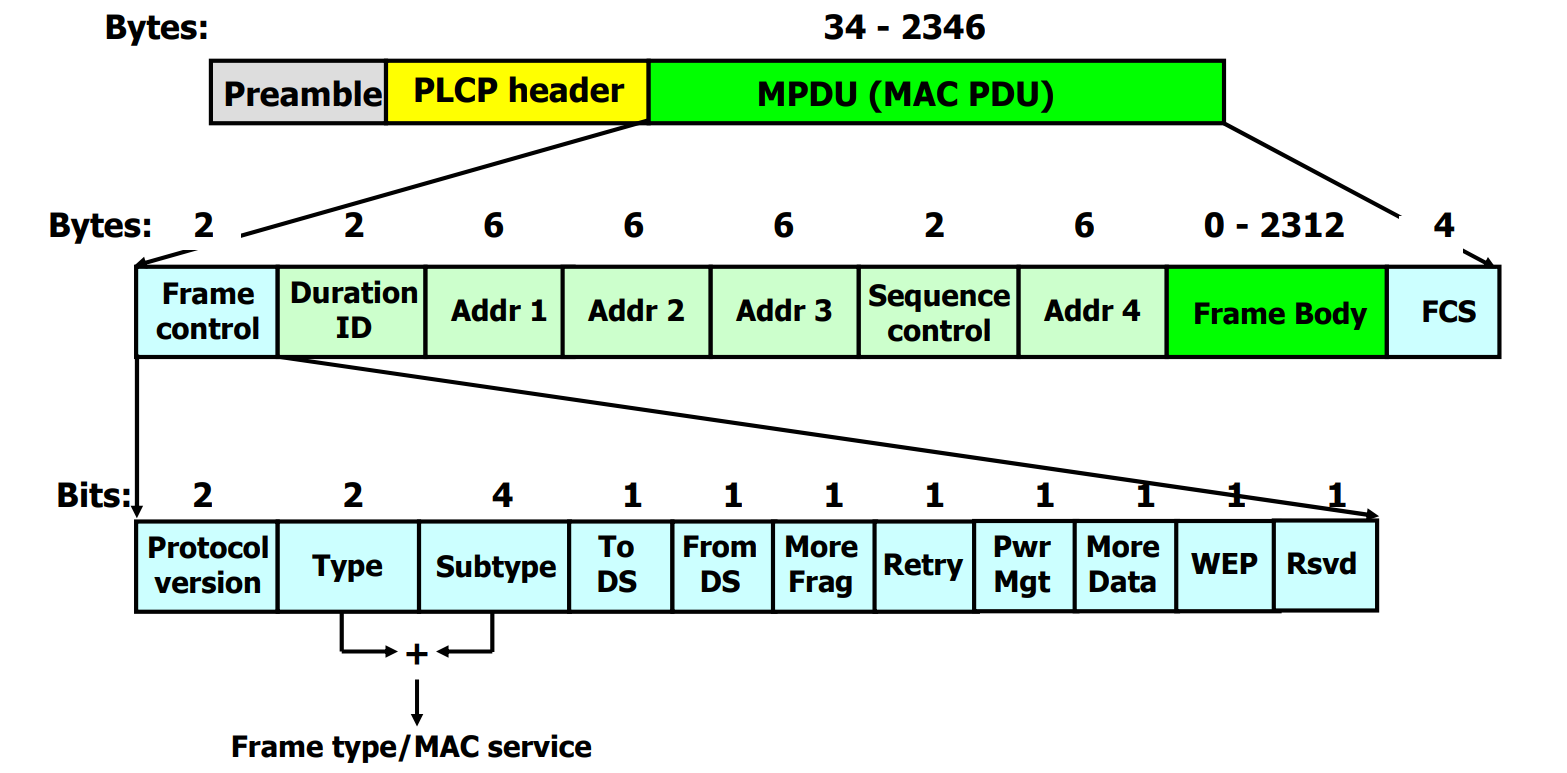
\includegraphics[width=\linewidth]{frame-macro.png}
  \caption{Estrutura de Quadro 802.11}
  \label{fig:frame-macro}
\end{figure}

\par Além das informações de endereço e os próprios dados transmitidos, um quadro contém informações de controle. Tais informações de controle possuem diversas funcionalidades, tais como: versão do protocolo 802.11, tipo do frame, se é uma retransmissão, controle de energia, ordenação, etc.
\par Neste trabalho, serão descritas especificamente as informações de tipo e subtipo do quadro.

\section*{Tipo do Quadro}

\par O Tipo do Quadro é um valor de 2 bits que indica se este é:

\begin{description}[align=left]
  \item [Quadro de Administração (00):] Tratam de informações referentes à descoberta de rede, autenticação e associação.
  \item [Quadro de Controle (01):] Tratam de informações de controle de fluxo de informações.
  \item [Quadro de Dados (10)] 
  \item [Reservado para Uso Futuro (11)]
  \end{description}

\section*{Subtipo do Quadro}

\par O Subtipo do Quadro é um valor de 4 bits que, combinado ao Tipo do Quadro, indicam do que se trata a informação contida no Corpo do Quadro.

\subsection*{Quadro de Administração (00)}

\begin{description}[align=left]
\item [0000 - Requisição de Associação:] A estação (STA) envia um pedido de associação para que se dê início à transmissão de dados.
\item [0001 - Resposta de Associação:] Resposta do Ponto de Acesso (AP) à Requisição de Autenticação.
\item [0010 - Requisição de Reassociação:] A STA envia um pedido de reassociação sempre que há perda na conexão, mas está já está localizada na Tabela de Endereços.
\item [0011 - Resposta de Reassociação:] Resposta do AP à Requisição de Reassociação.
\item [0100 - Requisição de Sondagem:] A STA envia um \textit{broadcast} requisitando que os APs com SSID público se identifiquem.
\item [0101 - Resposta de Sondagem:] Resposta dos APs à Requisição de Sondagem.
\item [0110-0111 - Reservado para Uso Futuro] 
\item [1000 - Beacon:] São transmitidos periodicamente por APs com informações à respeito da rede.
\item [1001 - Anúncio de Mensagem de Indicação de Tráfego (ATIM):] Transmitido à STAs em estado de Economia de Energia, informando que estas devem sair do estado de suspensão por determinado tempo para que possa receber dados em \textit{buffer}.
\item [1010 - Desassociação:] Indica que a comunicação com uma STA foi interrompida, por qualquer razão: inatividade, perda de sinal, perda excessiva de quadros, etc.
\item [1011 - Autenticação:] A STA envia um Quadro de Autenticação com informações de autenticação na rede.
\item [1100 - Desautenticação:] Indica que a STA não está mais autenticada, por qualquer razão: mudança de senha, mudança de canal, quantidade de STAs conectadas, etc.
\item [1101-1111 - Reservado para Uso Futuro] 
\end{description}

\bigbreak

\subsection*{Quadro de Controle (01)}

\begin{description}[align=left]
\item [0000-1001 - Reservado para Uso Futuro] 
\item [1010 - Power Save (PS)-Poll:] Requisição para que a STA entre em estado de economia de energia. No Corpo do Quadro estão informações do intervalo pelo qual a STA permanecerá neste estado.
\item [1011 - Requisição para Enviar (RTS):] Encaminhado pela STA quando há dados em \textit{buffer} para serem enviados.
\item [1100 - Livre para Enviar (CTS):] Enviado pelo AP indicando que a STA está livre para transmitir.
\item [1101 - Confirmação (ACK)]
\item [1110 - Fim do Período Livre-de-Contenção (CF)-End]
\item [1111 - CF-End + CF-ACK:] Enviado pelo AP, indicando o fim do período livre de contenção e indicando que recebeu o último quadro encaminhado por uma STA.
\end{description}

\bigbreak

\subsection*{Quadro de Dados (10)}

\begin{description}[align=left]
\item [0000 - Dados]
\item [0001 - Dados + CF-ACK:] Contém Dados e uma Confirmação que o último quadro encaminhado foi recebido.
\item [0010 - Dados + CF-Poll:] Durante o Período Livre-de-Contenção, o AP encaminha dados para uma estação, e encaminha em \textit{broadcast} uma requisição para que estações que possuam dados em \textit{buffer} se identifiquem.
\item [0011 - Dados + CF-ACK + CF-Poll:] Durante o Período Livre-de-Contenção, o AP encaminha dados para uma estação, encaminha em \textit{broadcast} uma requisição para que estações que possuam dados em \textit{buffer} se identifiquem, e também confirma que o último quadro encaminhado foi recebido.
\item [0100 - Função Nula (Sem Dados):] Quadros sem Dados são encaminhados por STAs para indicar ao AP sobre o estado atual de Economia de Energia. Caso possua o bit de Estado de Energia "0", indica que a STA está Online. Se o bit de Estado de Energia for "1", indica que a STA estará desligada temporariamente.
\item [0101 - CF-ACK (Sem Dados):] O AP confirma que o último quadro encaminhado foi recebido.
\item [0110 - CF-Poll (Sem Dados):]  O encaminha em \textit{broadcast} uma requisição para que estações que possuam dados em \textit{buffer} se identifiquem.
\item [0111 - CF-ACK + CF-Poll (Sem Dados):] O AP confirma que o último quadro encaminhado foi recebido e encaminha em \textit{broadcast} uma requisição para que estações que possuam dados em \textit{buffer} se identifiquem.
\item [1000-1111 - Reservado para Uso Futuro]
\end{description}

\end{document}
